%----------------Cap_04----------------%

\chapter{CITAÇÕES E REFERÊNCIAS}

Todo trabalho acadêmico é resultado de uma pesquisa e investigação. Uma importante etapa de toda pesquisa é a pesquisa bibliográfica com o intuito de saber se o tema do trabalho já foi publicado por outro autor e que metodologias foram utilizadas.

De acordo com as normas  \citeonline{nbr6023} e \citeonline{nbr10520}, todas as fontes utilizadas para a pesquisa devem ser devidamente citadas e referenciadas no trabalho final.


\section{Criando um arquivo bibtex para as referências}


Neste modelo de dissertação, as referências bibliográficas são produzidas utilizando o bibTeX \cite{bibtex-org}. Trata-se basicamente de um arquivo em separado do arquivo mestre que serve como um ``banco de dados'' no qual estão salvas as informações catalográficas de todas as referências da pesquisa. 

O arquivo bibTeX tem extensão .bib e no caso deste modelo está salvo com o nome \textbf{bibliografia.bib}.

Na dissertação, as referências são produzidas por meio do comando 
\begin{verbatim}
\bibliography{nome-do-arquivo-bibtex}
\end{verbatim}
escrito no início do arquivo \textbf{Postextual.tex}.

Uma das principais vantagens do bibTeX, é que ainda que o arquivo banco de dados tenha uma grande quantidade de referências, somente aquelas que foremefetivamente \textbf{citadas} no texto serão impressas.

Cada entrada no arquivo bibTeX deve ter a estrutura:
\begin{verbatim}
@tipo{etiqueta,
propriedade1 = {valor1},
propriedade2 = {valor2},
propriedade3 = {valor3},
...
}
\end{verbatim}
onde \textbf{tipo} se refere ao tipo de referência: artigo, livro, etc. O principais tipos permitidos são:
\begin{verbatim}
article
book
conference
manual
phdthesis
misc
\end{verbatim}

A \textbf{etiqueta} serve como um ``apelido'' para a entrada. Usando essa etiqueta, é possível fazer a citação no texto com, por exemplo, o comando \verb!\cite{etiqueta}!. As \textbf{propriedades} se referem aos elementos que caracterizam a referência. Por exemplo, a propriedade \verb!author! indica o nome do autor, a propriedade \verb!title! indica o título da obra referenciada, a propriedade \verb!address! indica o local (cidade, estado) onde a obra foi publicada.

Usando o editor Texmaker, cada nova entrada no arquivo \textbf{bibli\_profmat.bib} clicando-se em \textsl{bibliografia} na barra de ferramentas, escolhendo-se \textsl{Bibtex} na caixa de seleção e então escolhendo-se o tipo de entrada mais adequado a obra referenciada. O processo é ilustrado na figura abaixo:
	\begin{figure}[H]
	\centering
	\caption{Criando referências com bibTeX}
	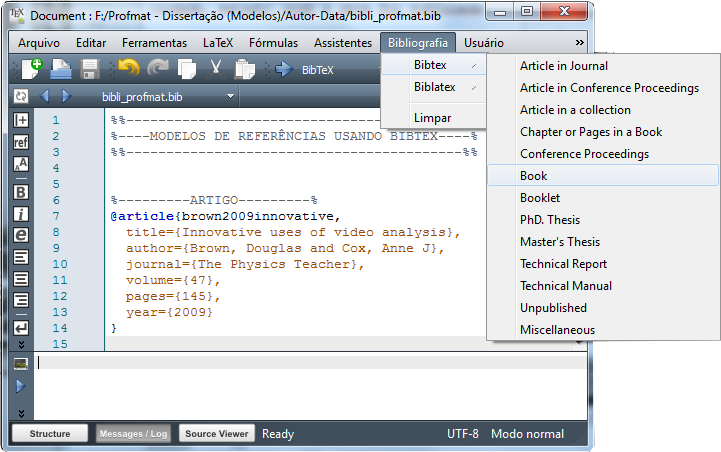
\includegraphics[scale=0.45]
	{img/fig08.png}\label{fig08}\\
	FONTE: Autor (2015)
	\end{figure}


 Como exemplo, observe duas referências escritas no arquivo \textbf{bibliografia.bib}:
\begin{verbatim}
@Manual{nbr14724,
title = {ABNT NBR 14724:2011},
subtitle={Informação
e documentação - trabalhos acadêmicos - apresentação},
author = {ABNT},
address = {Rio de Janeiro},
year = {2011},
}

@Book{AL_hefez,
author = {Abramo Hefez and Cecília de Souza Fernandez},
title = {Introdução à Álgebra Linear},
publisher = {SBM},
series = {Coleção Profmat},
year = {2013},
address = {Rio de Janeiro},
edition = {1},
}
\end{verbatim}

Caso no texto sejam inseridos os comandos \verb!\cite{nbr14724}! e \verb!\cite{AL_hefez}!, uma lista de referências será criada conforme ilustra a figura a seguir:
	\begin{figure}[H]
	\centering
	\caption{Criando referências com bibTeX, resultado em tela}
	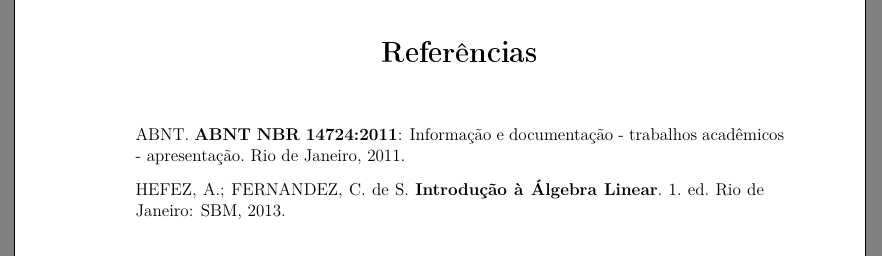
\includegraphics[scale=0.45]
	{img/fig09.png}\label{fig09}\\
	FONTE: Autor (2015)
	\end{figure}


\section{Modelos de citação}

A NBR 10520 define uma citação como uma ``menção de uma informação extraída de outra fonte'' \cite[p.~1]{nbr10520}. A referida norma ainda define os tipos de citação:
\begin{itemize} 
	\item citação direta, quando ocorre a transcrição do texto tal qual está escrino na fonte original;
	\item citação indireta, quando cria-se um texto baseado na obra consultada; e
	\item citação de citação, quando se faz uma citação, direta ou indireta, de um texto ao qual se teve acesso apenas por meio de outro autor,
\end{itemize}
bem como orienta sobre as regras de apresentação das citações no texto.


\subsection{Citação direta}

A norma NBR 10.520 classifica as citações diretas quanto ao tamanho em citações de \textbf{até três linhas} e citações \textbf{com mais de três linhas}. 


\subsubsection{Citação direta com até três linhas}

No caso de citações com \textbf{até três linhas}, as citações ``[$\cdots$] devem estar contidas entre aspas duplas. As aspas simples são
utilizadas para indicar citação no interior da citação'' \cite[p.~2]{nbr10520}. 



A figura abaixo ilustra como escrever em latex uma citação direta com até três linhas:
	\begin{figure}[H]
	\centering
	\caption{Citações com até três linhas}
	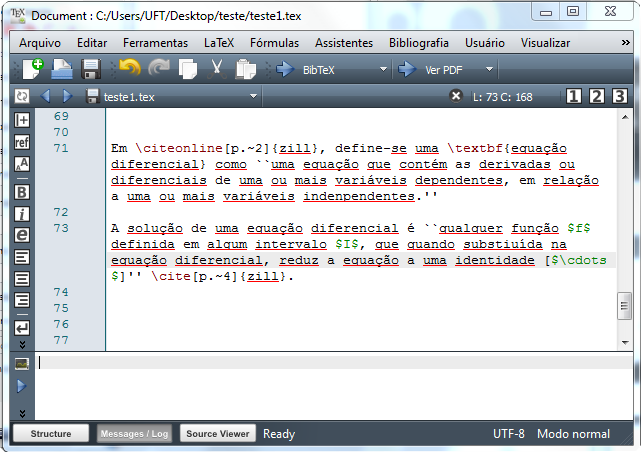
\includegraphics[scale=0.45]
	{img/fig10.png}\label{fig10}\\
	FONTE: Autor (2015)
	\end{figure}

O resultado em PDF é mostrado na Figura \ref{fig11}:
	\begin{figure}[H]
	\centering
	\caption{Citações com até três linhas, resultado em tela}
	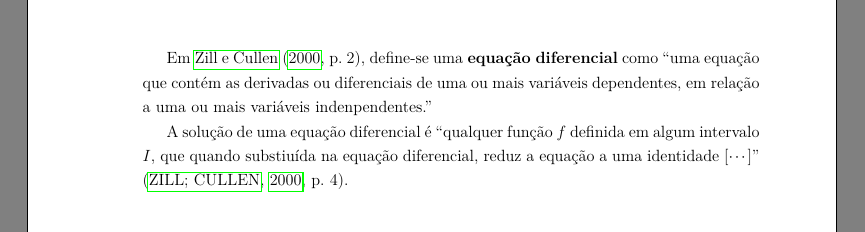
\includegraphics[scale=0.45]
	{img/fig11.png}\label{fig11}\\
	FONTE: Autor (2015)
	\end{figure}
	
	Observe que foram utilizados dois comandos. O comando \verb!\citeonline[]{}! insere a fonte dentro do texto. O nome do autor da fonte aparece com apenas a primeira letra maiúscula. O ano da obra e a página(s) de onde foi retirada a citação estão entre parêntesis. O número da página é inserido na opção \verb![p.~2]!.
	
	O comando \verb!\cite[]{}! insere a fonte, ano da obra e página(s) consultadas entre parêntesis.
	
\subsubsection{Citação direta com mais de três linhas}

Para criar citações com mais de três linhas em LaTeX, é necessário usar o ambiente \texttt{citacao}, conforme exemplo a seguir:
	\begin{figure}[H]
	\centering
	\caption{Citações com mais de três linhas}
	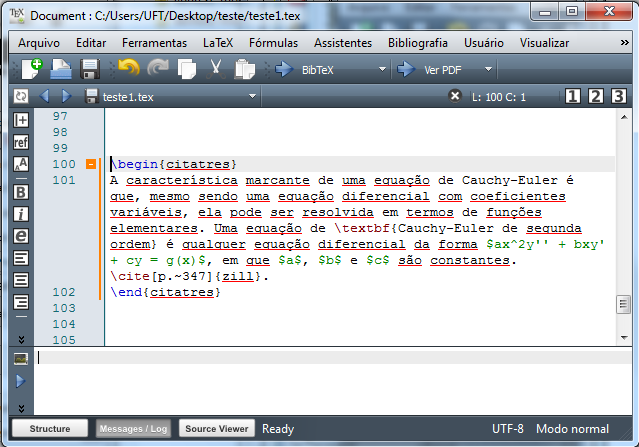
\includegraphics[scale=0.45]
	{img/fig12.png}\label{fig12}\\
	FONTE: Autor (2015)
	\end{figure}
O resultado é mostrado a seguir:
\begin{citacao}
A característica marcante de uma equação de Cauchy-Euler é que, mesmo sendo uma equação diferencial com coeficientes variáveis, ela pode ser resolvida em termos de funções elementares. Uma equação de \textbf{Cauchy-Euler de segunda ordem} é qualquer equação diferencial da forma $ax^2y'' + bxy' + cy = g(x)$, em que $a$, $b$ e $c$ são constantes. \cite[p.~347]{zill}.
\end{citacao}

\subsection{Citação indireta}

As citações indiretas são produzidas em LaTeX utilizando-se os mesmos comandos descritos acima para citação direta com até três linhas. Como exemplo, observe a figura abaixo:
	\begin{figure}[H]
	\centering
	\caption{Citação indireta, comando LaTeX}
	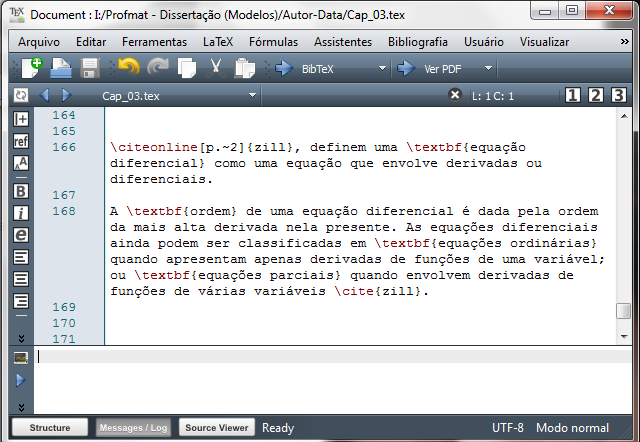
\includegraphics[scale=0.45]
	{img/fig14.png}\label{fig14}\\
	FONTE: Autor (2015)
	\end{figure}

O resultado é mostrado abaixo:
	\begin{figure}[H]
	\centering
	\caption{Citação indireta, em tela}
	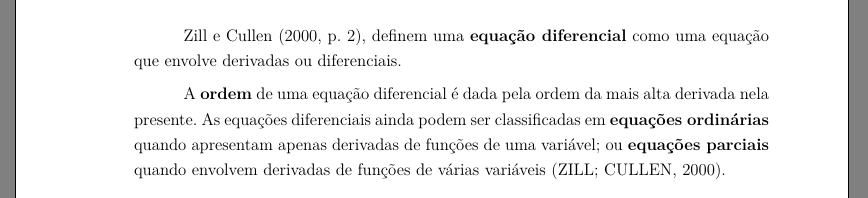
\includegraphics[scale=0.45]
	{img/fig15.png}\label{fig15}\\
	FONTE: Autor (2015)
	\end{figure}
	


\section{Compilando um documento com citações e referências}
 

Para produzir o documento em PDF (para impressão ou leitura em tela do computador), deve-se compilar o código-fonte em LaTeX. Utilizando o editor TexMaker esta ação é realizada clicando no botão \textbf{compilar} na barra de edição do programa conforme ilustra a figura abaixo:
	\begin{figure}[H]
	\centering
	\caption{Compilando o documento LaTeX}
	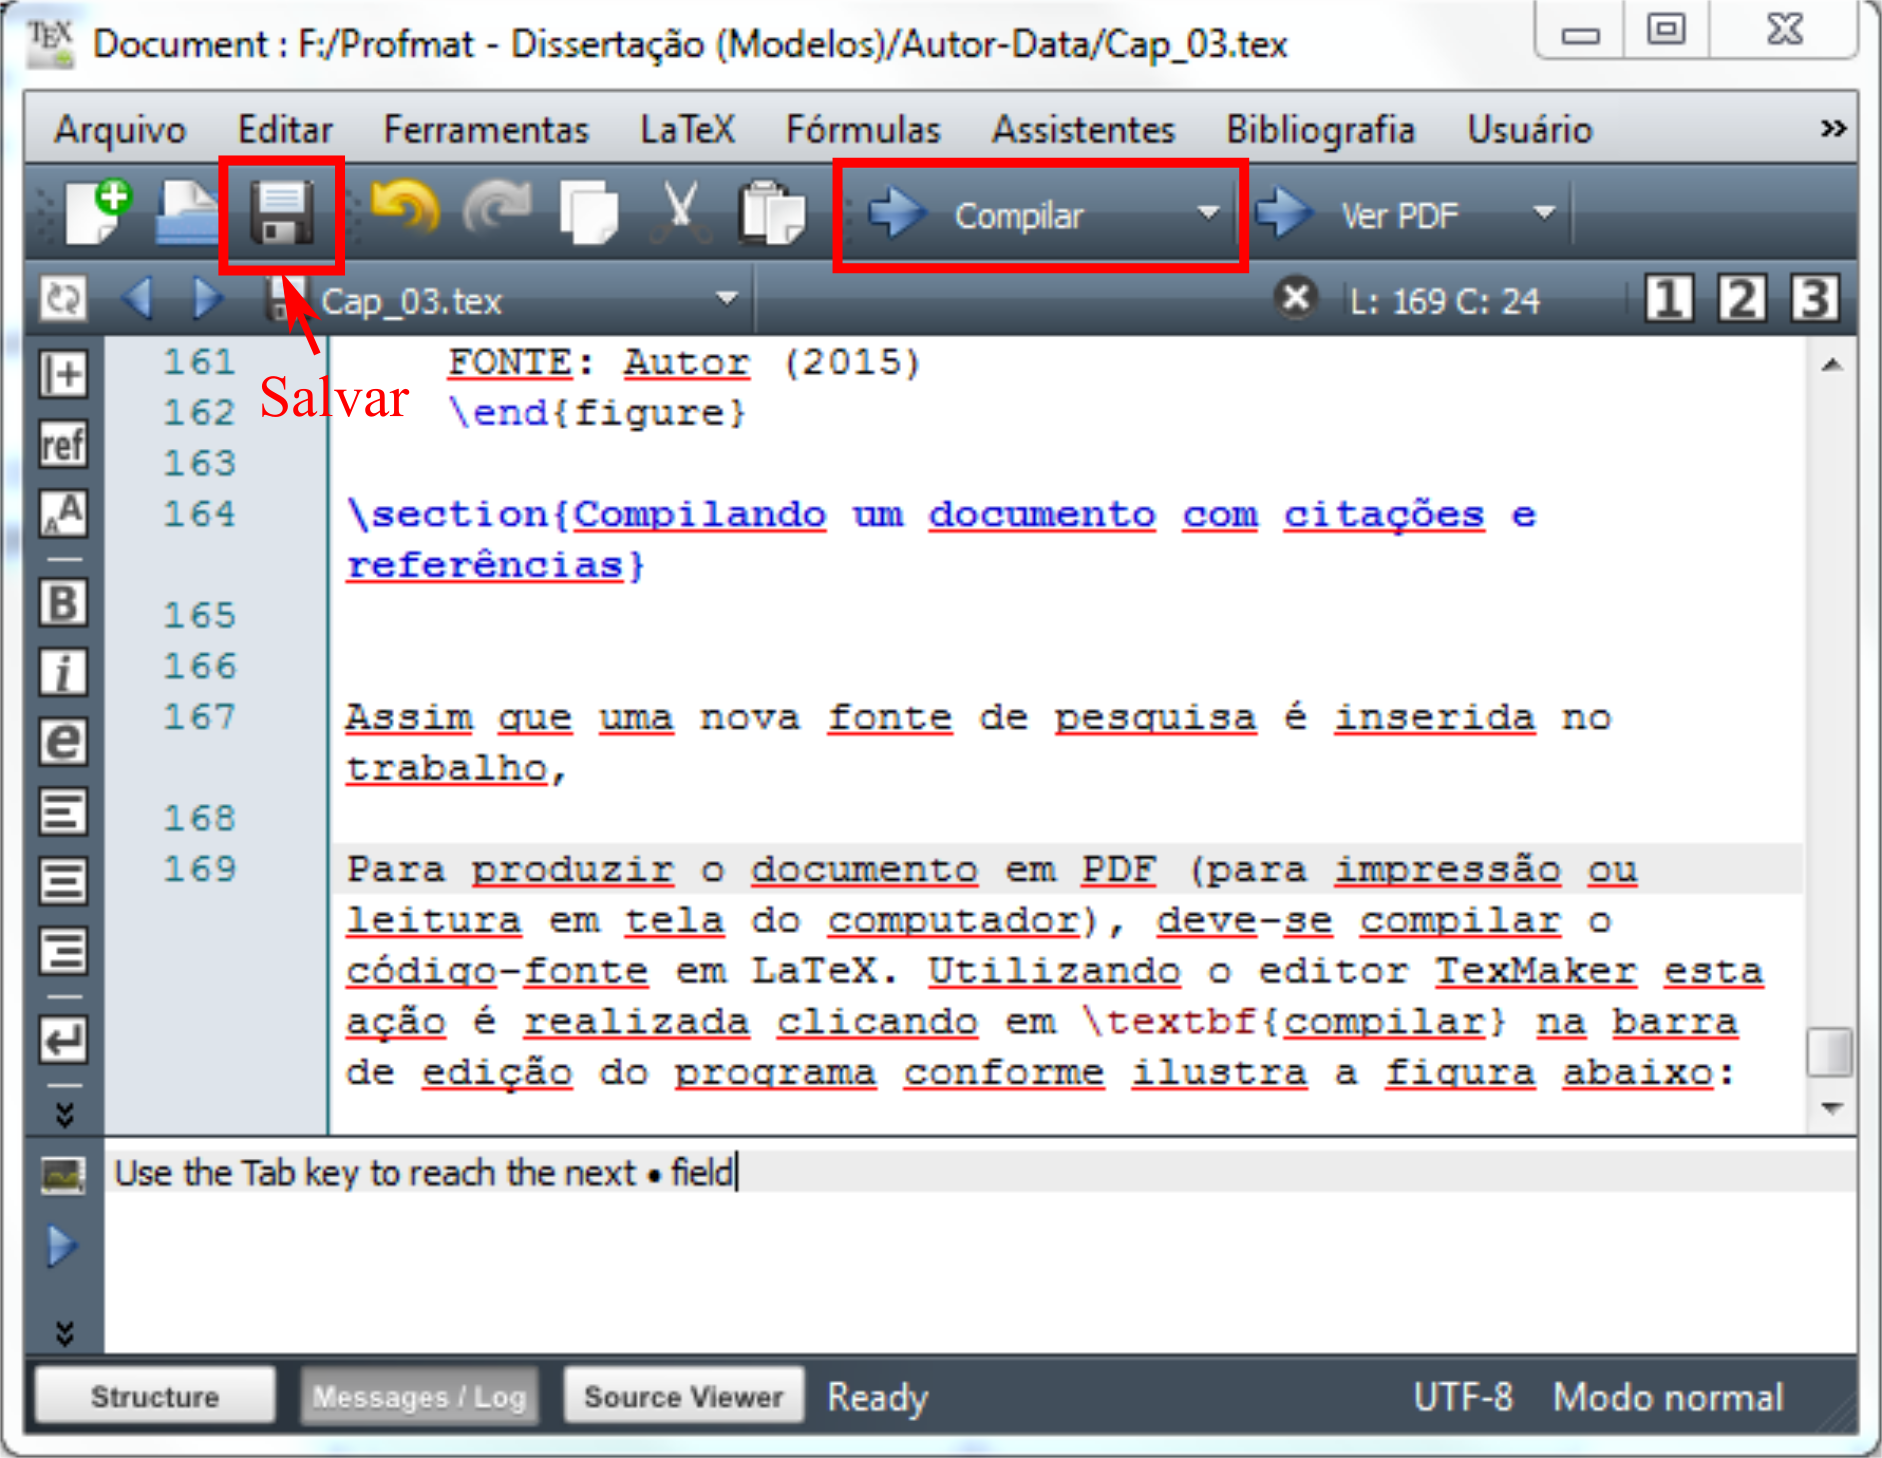
\includegraphics[scale=0.25]
	{img/fig17.png}\label{fig17}\\
	FONTE: Autor (2015)
	\end{figure}
	Uma nova janela será aberta para visualização do resultado em PDF. Na pasta onde o trabalho está sendo salvo, o arquivo \textbf{nome-do-arquivo.pdf} também é atualizado conforme as novas informações inseridas.
	\begin{figure}[H]
	\centering
	\caption{Documento PDF após compilação LaTeX}
	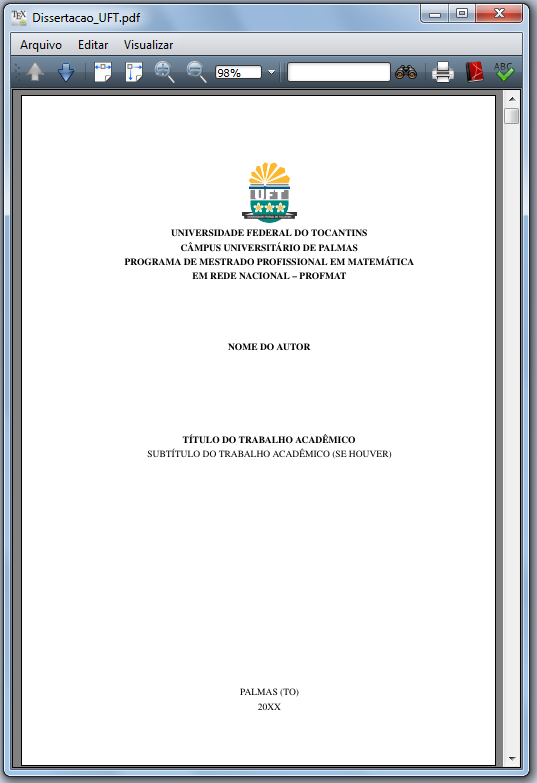
\includegraphics[scale=0.7]
	{img/fig18.png}\label{fig18}\\
	FONTE: Autor (2015)
	\end{figure}
	Neste ponto, uma observação importante. Quando o código-fonte LaTeX está dividido em arquivos menores, como é o caso deste modelo de dissertação, apenas o arquivo mestre (neste modelo, o arquivo \textbf{Dissertacao\_UFT.tex}) deve ser compilado. Os demais arquivos (\textbf{Pretextual.tex}, \textbf{Cap\_01.tex}, \textbf{Cap\_02.tex}, ...) são apenas salvos.
	
	Além disso, assim que uma nova fonte de pesquisa é inserida no trabalho, nem sempre ela aparecerá de imediato no arquivo em PDF. Isso ocorre pois, antes de compilar o código-fonte, é preciso informar ao programa para atualizar o banco de dados bibTeX. Para realizar este procedimento, deve-se clicar na seta ao lado do botão \textbf{compilar}. Aparecerá uma caixa de opções na qual deve-se escolher a opção \textbf{BibTeX}. Após isso, clica-se novamente em \textbf{compilar} para visualizar o arquivo PDF.
	\begin{figure}[H]
	\centering
	\caption{Atualizando banco de dados BibTeX}
	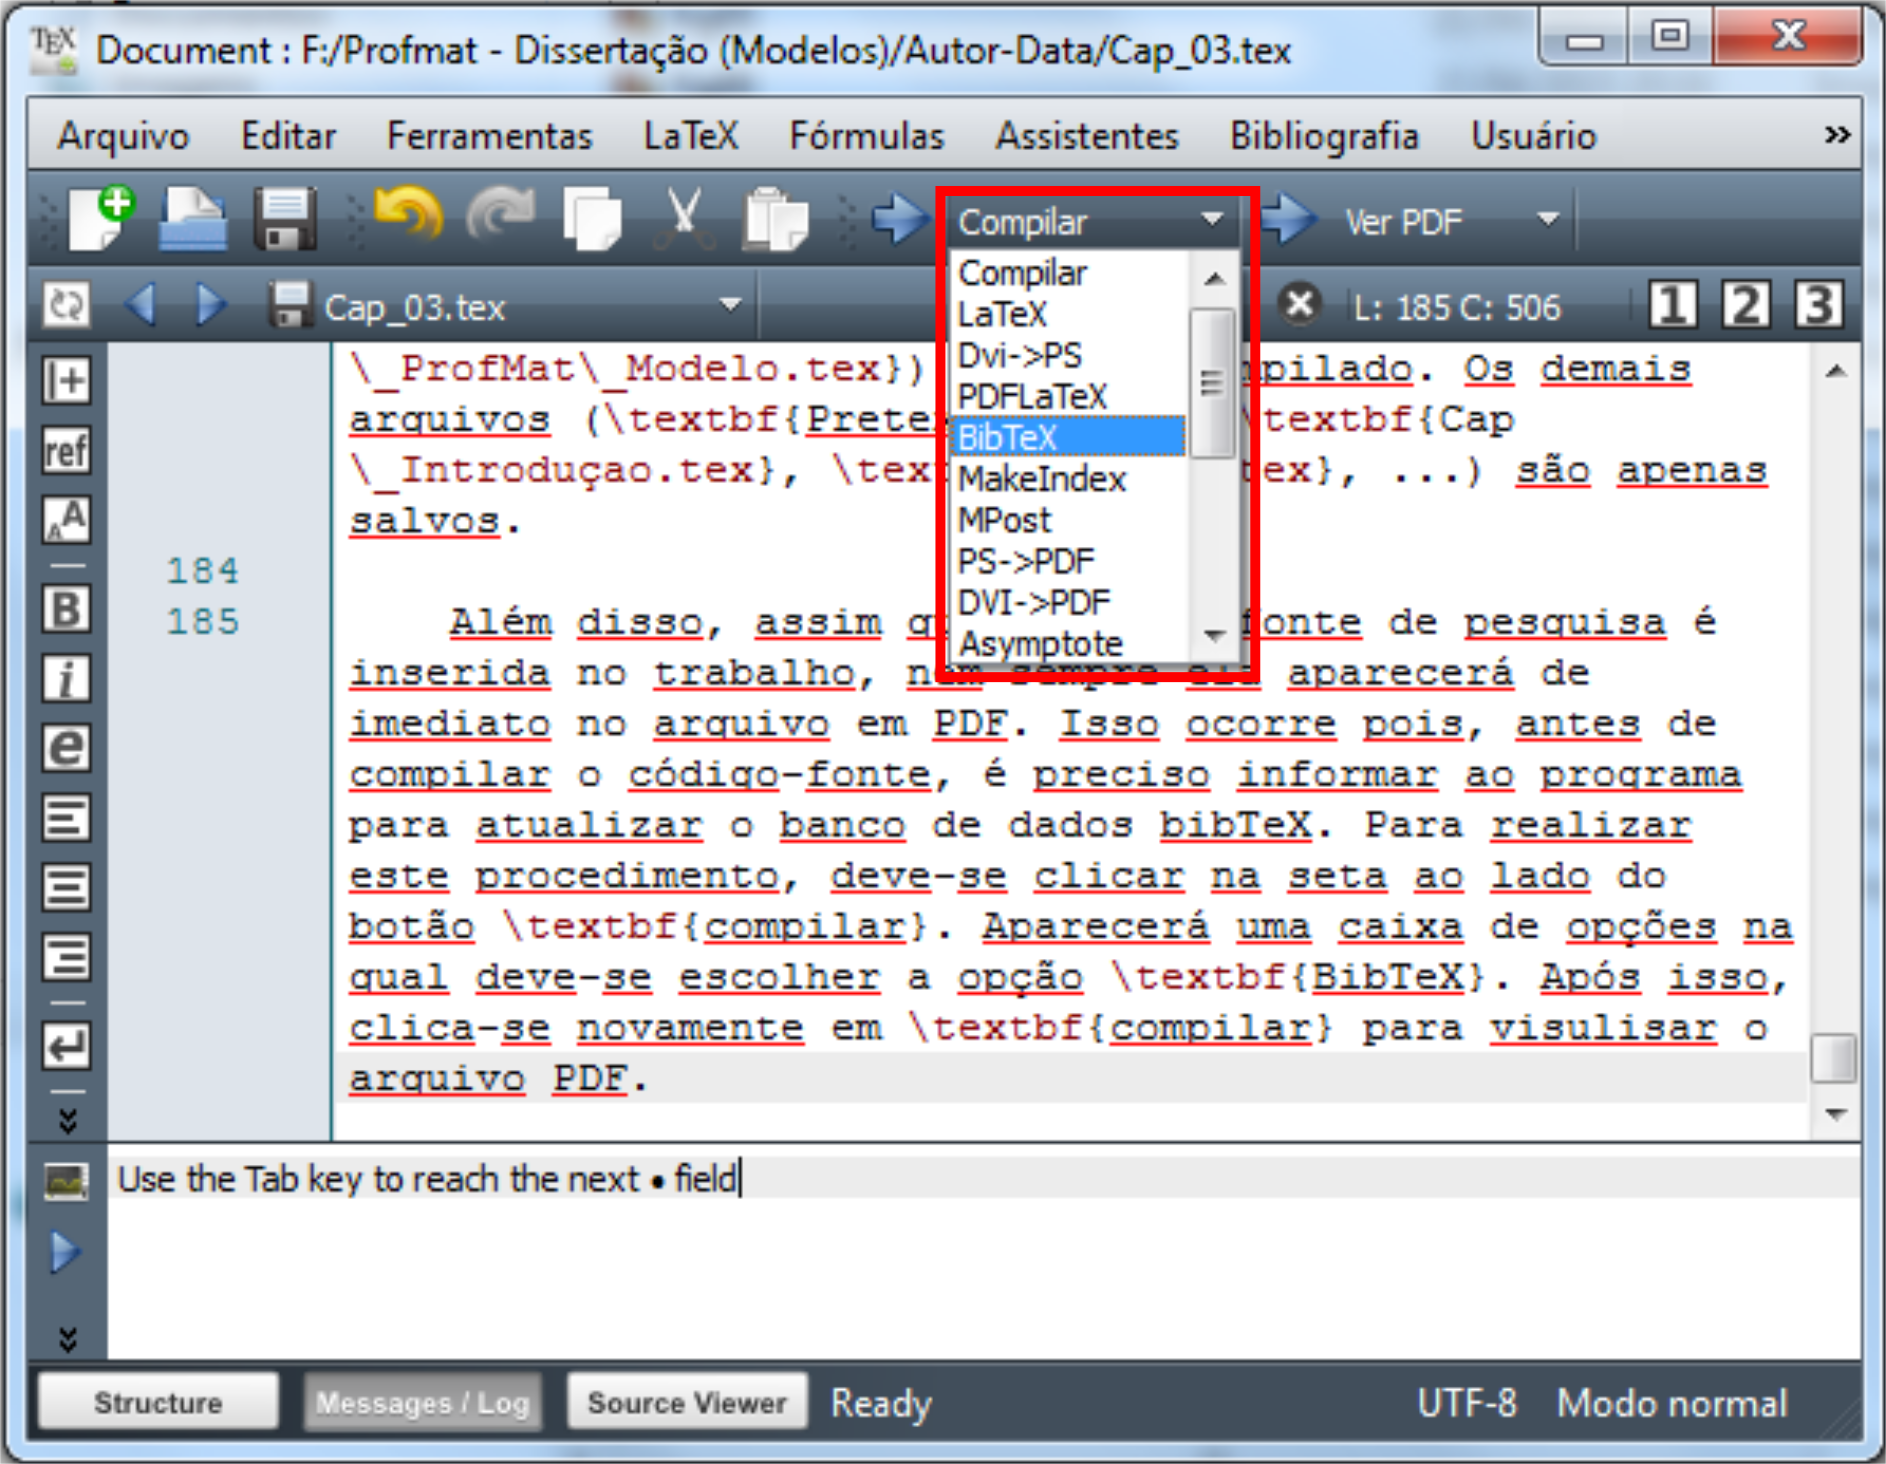
\includegraphics[scale=0.25]
	{img/fig19.png}\label{fig19}\\
	FONTE: Autor (2015)
	\end{figure}
	
	Os procedimentos descritos acima podem ser facilitados e agilizados com o uso de atalhos de teclado. Para um lista completa de atalhos LaTeX no TexMaker, basta clicar em \textbf{Ferramentas} na barra de ferramentas. Para compilar um documento, clique na tecla \keystroke{F1} e para atualizar a lista de referências BibTeX, clique em \keystroke{F11}.
	

